\chapter{Литературный обзор} \label{chapt1}

Для того чтобы отслеживать активность любого объекта, можно представить что в каждый момент времени у этого объекта существует состояние. На шкале времени состояние объекта может меняться, таким образом мы поймём что объект был неподвижен или наоборот, совершал активность - в нашем случае смену состояния.

Состояние объекта можно описать непрерывными функциями - как, например, координаты тела в пространстве. А можно дискретными, когда количество состояний ограничено. Пример - собака смотрит в камеру, в сторону, вверх.

% два изображения: машина на координатной оси, человек на 2 кадрах расположен анфас, в профиль
% картинка с Pose estimation и 3D pose estimation
\begin{figure}[ht] 
  \center
  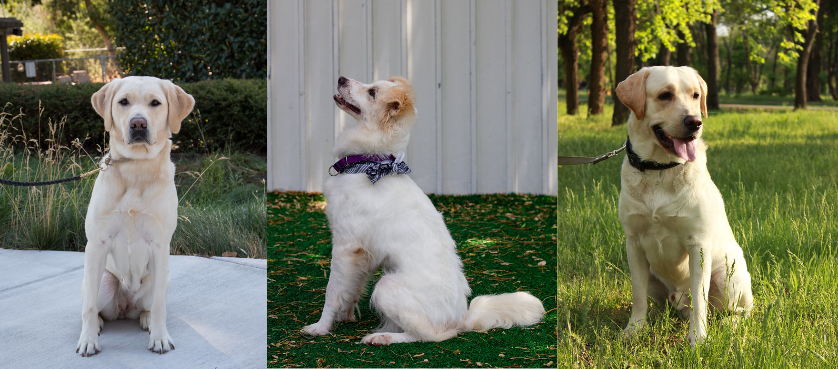
\includegraphics [width=\textwidth] {front_side_view_dog}
  \caption{Cобака в профиль, анфас и 3/4} 
  \label{img:front_side_view_dog}  
\end{figure}

Для отслеживания базовой активности собак, нам подойдут оба эти варианта. Возможно отслеживать как координаты каждой конечности собаки - лап, хвоста, туловища, головы. Такая задача в иностранной литературе будет называться Pose Estimation и подразумевает возвращение некоторой функцией координат тела в двумерном пространстве кадра. Если же требуется получить вектор перемещения и поворота относительно камеры, такую задачу называют 3D Pose Estimation.

% картинка c 3D pose estimation
\begin{figure}[ht] 
  \center
  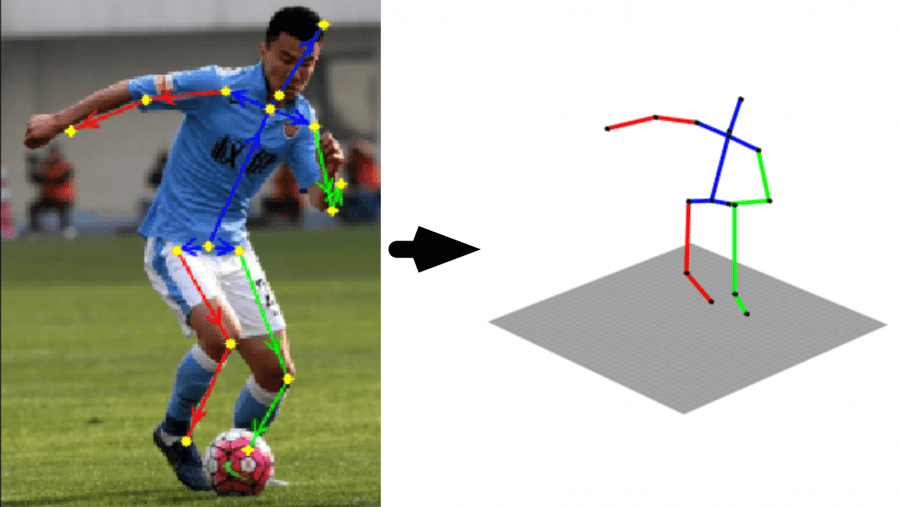
\includegraphics [width=\textwidth*2/3] {3dposeest}
  \caption{3D Pose Estimation} 
  \label{img:3dposeest}  
\end{figure}

Так как конечная цель этой работы - классифицировать простые активности собаки, например, когда собака сидит, стоит или лежит - задачу Pose Estimation решать необязательно, но она может значительно упростить дальнейшую классификацию, так как позволить отбросить избыточную визуальную информацию, которую мы имеем на фотографии и оставить только информацию о расположении конечностей относительно друг друга.


\section{Эмоции собак} \label{sect1_1}
%Section start
% Изначальная миссия этого исследования, выходящего за рамки данной работы, анализировать эмоции собаки. Но для понимания даже базовых эмоций требуется уметь считывать базовые сигналы как поджатый, или наоборот, торчащий хвост. Либо оскал,  

Большинство людей интуитивно понимает основные значения телодвижений собаки и может определить, когда их собака счастлива, напугана или зла. Тем не менее язык тела человека и язык тела собаки очень различаются. Поза, выражение морды и телодвижения, которые мы интерпретируем как определенные эмоции, для вашей собаки могут означать нечто иное. По сути, язык тела собаки состоит из множества различных элементов, которые включают:

\begin{itemize}
    \item Выражение морды.
    \item Положение ушей.
    \item Положение и движение хвоста.
\end{itemize}

Эти аспекты всегда следует интерпретировать вместе, так как это единственный способ точно «расшифровать» эмоции вашей собаки.


\subsubsection{Хвост и уши собаки: выражение эмоций}

Собака сообщает о своих эмоциях и намерениях определенными телодвижениями, будь то общее поведение животного или движения определенной части тела. Однако хвост и уши собаки — это две части тела, на которые следует обращать особое внимание для понимания языка тела животного.\cite{DogSignals}

\subsection{Собачий хвост}

%фотография с разными хвостами: круглый, короткий, длинный. Например, хаски, корги и хз
Как это часто бывает с животными, хвост каждой отдельной собаки говорит о чем-то своем. У некоторых собак хвосты большие и пушистые, у других — хвосты скручены в кольцо и лежат на спине, у третьих — хвосты куцые и мало о чем могут рассказать. Собаки таких пород, как уиппет, ирландский волкодав или борзая, обычно держат хвосты между ног, а значит, они не станут выражать волнение, пряча свои хвосты, как это делают собаки большинства пород. При интерпретации сигналов, подаваемых хвостом, важно всегда учитывать контекст, а также характер и породу отдельной собаки!

\subsubsection{Виляние хвостом}
Одним из самых широко известных является факт, что, виляя хвостом, собака выражает свою радость. Однако в действительности виляние хвостом — не всегда верный признак радости животного. Такое поведение лишь означает, что собака заинтересована во взаимодействии, и только в сочетании с другими элементами языка тела виляние хвостом может быть интерпретировано как радость или беспокойство.

Скорость, с которой собака виляет хвостом, также может послужить ключом к разгадке ее эмоций. Например, быстрое и бодрое виляние обычно является хорошим, дружелюбным жестом, в то время как медленное виляние может быть признаком того, что собака насторожена и взволнована.

\subsubsection{Виляние напряженным хвостом}
Если ваш пес напряжен и скованно виляет хвостом из стороны в сторону, это может быть признаком агрессивного поведения или беспокойства. Иногда это называют «хвост флажком» (не путать с английским термином «флагинг», означающим другое движение хвостом), и он является показателем течки у сук.

\subsubsection{Хвост, зажатый между ног}

%фотка спрятанного хвоста
\begin{figure}[ht] 
  \center
  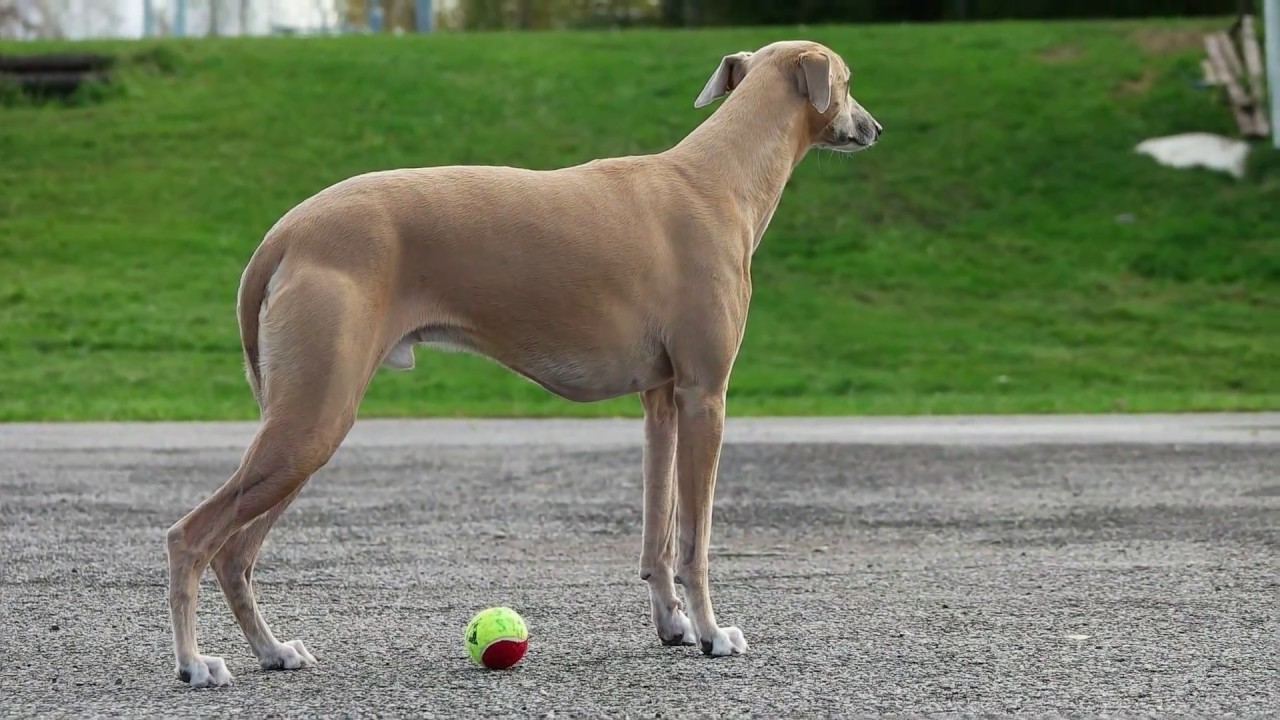
\includegraphics [width=\textwidth/2] {tail-between-legs}
  \caption{Хвост, зажатый между ног} 
  \label{img:tail-between-legs}  
\end{figure}

Если хвост собаки зажат между задними лапами, это означает, что она обеспокоена или напугана. В зависимости от внешних обстоятельств, позы и языка тела собаки, такое поведение может перерасти в оборонительную агрессию, поэтому в подобной ситуации важно подходить к собаке спокойно и осторожно.

Тревожные и пугливые собаки прячут хвост между ног, когда они находятся в незнакомой для них среде или встречают новых людей или животных. Обычно это признак их неуверенности и беззащитности. Послушная собака чаще держит хвост между ног, особенно когда она общается с другими собаками или хочет показать готовность подчиняться, например, в ситуации, когда ее привели к ветеринару на обследование, или после того, как она в чём-то провинилась.

\subsection{Собачьи уши}
\begin{figure}[ht] 
  \center
  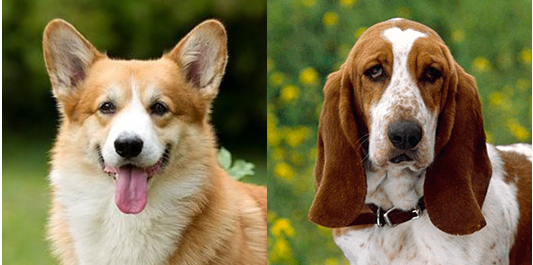
\includegraphics [width=\textwidth/2] {ears-different}
  \caption{У некоторых пород уши острые, у других свисающие} 
  \label{img:ears-different}  
\end{figure}
%кроп ушей острых у корги и бассет-хаунда
Как и в случае с хвостами, форма и тип ушей собаки имеют большое значение в том, как она будет их держать при общении. Не стоит ожидать от собак, например, породы бассет-хаунд, что они будут держать свои уши в вертикальном положении, как это делают породы собак с оттопыренными ушами. В то же время, независимо от формы, размера и типа ушей собаки, можно многое узнать о ее эмоциях и намерениях, научившись распознавать значение положения ушей питомца.

\subsubsection{Уши, направленные назад}
%найти такую фотку
Если уши собаки слегка направлены назад и при этом она радостно виляет хвостом, значит, собака настроена дружелюбно. Однако, если уши плоские и прижаты к спине или по бокам головы, собака определенно сигнализирует о страхе. В зависимости от языка тела собаки с прижатыми ушами ее поведение можно интерпретировать как выражение покорности или наоборот, предупреждение о возможном нападении.

\subsubsection{Заостренные уши}
Всякий раз, когда собака испытывает любопытство или настороженность, она поднимает уши вверх, после чего нередко задирает голову. Более того, собаки слегка направляют уши в сторону объекта или человека, который пробудил в них любопытство.

\subsection{Чтение языка тела собаки}

Язык тела собаки нельзя понять правильно, если при его интерпретации также не учитывать контекст и другие сигналы собаки. Например, оскал может означать радость, подчинение или агрессию — все зависит от остальных элементов языка тела.

Вот некоторые распространённые сигналы, которые обычно передают собаки.

\subsubsection{Выражения морды}

\textbf{Зевание}. Оказывает успокаивающее действие. Если собака не собирается вздремнуть, зевота может указывать на то, что она испытывает стресс или хочет избавиться от переживаний.

\textbf{Взгляд, опущенный вниз}. Собаки не особо любят прямой зрительный контакт, однако если они прожили с людьми долгое время, то начинают понимать, что взгляд не обязательно означает вызов. Отводя глаза, собака, в соответствии с собачьими привычками, просто пытается быть вежливой.

\textbf{Широко раскрытые глаза}. Когда собака отводит взгляд в сторону, концентрируя его на ком-то или чем-то, и виднеются белки (склеры) ее глаз, это признак встревоженности и беспокойства. 

\textbf{Открытый рот}. Такой растерянный вид означает, что пес доволен и расслаблен. Однако, если рот собаки открыт, когда рядом кто-то ест, это может быть просьба поделиться едой.
\begin{figure}[ht] 
  \center
  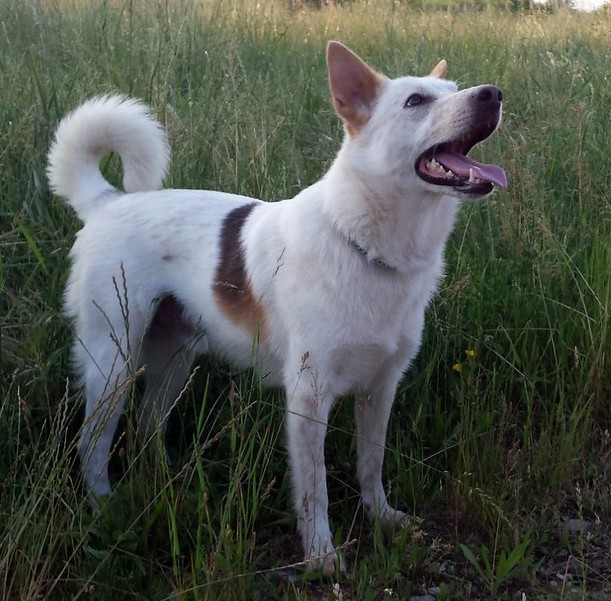
\includegraphics [width=\textwidth/2] {open-mouth}
  \caption{Открытый рот} 
  \label{img:open-mouth}  
\end{figure}
% две фотки тут

\textbf{Оскал / обнаженные зубы}. Этот сигнал может интерпретироваться по-разному в зависимости от ситуации. Он может быть проявлением покорности собаки или, если сопровождается рычанием, поднятой шерстью и защитной стойкой, признаком агрессивных намерений.

\textbf{Облизывание губ}. Если собака постоянно облизывает губы, не глядя при этом на еду, то таким образом она пытается передать чувство страха, стресса или нервозности. Собака может быть напугана или чувствует себя неуютно. В подобной ситуации это также может быть выражено другими сигналами, такими как учащенное дыхание, зажатый между ног хвост или широко раскрытые глаза.

\subsubsection{Положение тела собаки}
% на каждую секцию по фотке
\textbf{Расслабленное}. Расслабленность собаки можно определить, посмотрев на ее тело. Положение ее хвоста будет естественным, положение тела — непринужденным, а уши будут расслаблены или слегка направлены вверх. Собака не станет пристально смотреть или опускать глаза, а ее пасть будет расслаблена в уголках, челюсти сомкнуты или слегка приоткрыты.

\textbf{Возбужденное}. Собака быстро приближается к человеку или объекту, часто переходит на бег, прыжки и демонстрирует игривое настроение. При этом ее уши насторожены и подняты вверх, а хвост не успокаивается. Если пес чем-то особенно взволнован, он может также начать лаять или скулить.

\begin{figure}[ht] 
  \center
  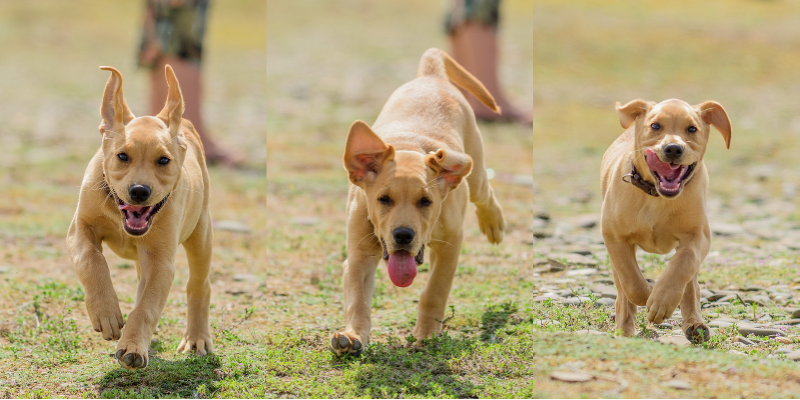
\includegraphics [width=\textwidth*2/3] {dog-run}
  \caption{Собака бежит в игривом настроении} 
  \label{img:dog-run}  
\end{figure}

\textbf{Напуганное}. Есть много способов, с помощью которых собака сообщает о страхе, и все они зависят от характера вашего питомца. Когда собаке страшно, она может нападать, прятаться и проявлять покорное поведение, а также искать утешения у своего хозяина. Большинство собак дрожит, прижимает тело к земле и зажимает хвост между ног.

\textbf{Игривое}. Собаку, которая хочет повеселиться, легко заметить. Типичная игривая стойка, когда передняя часть тела опущена на землю, а задние лапы выпрямлены, является недвусмысленным приглашением к игре как для хозяина, так и для другой собаки.

\textbf{Напряженное}. Если собака чувствует себя неуютно, она подаст об этом знак, напрягая и слегка опуская свое тело, а также направляя уши назад. У некоторых собак напряженная поза сопровождается зеванием или учащенным дыханием.

\textbf{Агрессивное}. Когда собака готовится к нападению, весь язык ее тела демонстрирует такое намерение. Агрессивные собаки имеют сосредоточенный или суженный взгляд, их тело напряжено, шерсть на затылке стоит дыбом, зубы обнажены в оскале, и можно услышать рычание. Тревожный лай и низкое рычание часто сопровождают агрессивное поведение собаки.


\section{Существующие датасеты} \label{sect1_2}
Насколько известно автору, по состоянию на Май 2020 года в открытом доступе содержатся только следующие наборы данных с изображениями собак:
\begin{enumerate}
  \item ImageNet \cite{imagenet} - Считается крупнейшим датасетом по классификации всего. Насчитывает более 1 миллиона изображений и больше 1000 классов изображений для классификации, начиная от машин, заканчивая собаками. Часто используется для оценки производительности систем компьютерного зрения а также для предобучения нейронных сетей при недостаточных данных.
  \item Stanford Dog Dataset \cite{KhoslaYaoJayadevaprakashFeiFei_FGVC2011} - Подраздел ImageNet. В нём содержится 20000 изображений собак 120 различных пород. Разметка осуществлялась для дальнейшей классификации собак по породам. Разные породы имеют различное количество изображений.
  \item OpenImageDataset \cite{openimages} - ближайший аналог ImageNet по назначению и реализации, за тем лишь исключением что он создавался с уклоном в детекцию объектов, поэтому все изображения там чуть большего размера, и на каждом изображения может быть несколько объектов, в том числе, разного класса. К каждому объекту прилагается информация о его ограничивающей рамке.
  \item DogCentric Activity Dataset \cite{yumi2014first} - Датасет с видеозаписями различных занятий собаки от лица самой собаки. Целью является классификация активности.
  \item Jena Action Recognition Dataset \cite{jena} - Коллекция видеозаписей с дистанционно управляемым роботом-собакой SONY ERS-7 Aibo. Создавалась для оценивания систем распозанавания. В ней есть видеозаписи, координаты ограничивающих рамок робота на каждом кадре и данные для калибровки.
\end{enumerate}
Все эти датасеты достаточно хорошо размечены. Важно заметить что в изображения собак в ImageNet, Stanford Dog Dataset и OpenImageDataset пересекаются, так что суммарно по этим трём датасетам имеется всего 20000 изображений собак, столько же сколько и в Stanford Dog Dataset.

\section{Методы решения задачи} \label{sect1_3}
В области определения позы животных проделано сильно меньше работы, чем в этой же области для людей. Причины очевидны:
\begin{itemize}
    \item Широкий потенциал применения
    \item Возможность использовать актёров
    \item Большое количество фотографий
\end{itemize}
\subsection{На людях} \label{subsect1_3_1}
Сейчас классификацию позы людей осуществляют с помощью так называемого Pose Estimation Tree. Целью зрения становится будто восстановить человеческий скелет по изображению. Для этого определяются важные подвижные узлы - joints. Обычно ими являются локти, колени и другие суставы. У человека всего порядка 200 таких узлов. При этом при решении большинства задач компьютерного зрения используется около 20.
\begin{figure}[ht] 
  \center
  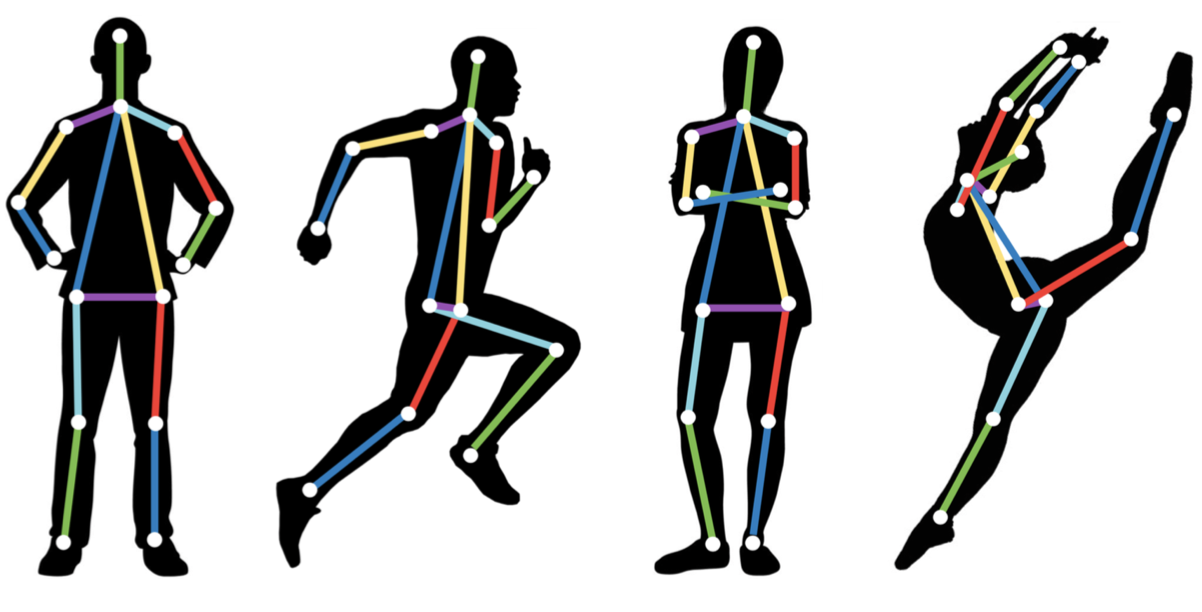
\includegraphics [width=\textwidth/2] {pose}
  \caption{Pose Estimation Tree} 
  \label{img:poseest}  
\end{figure}

Классические пакетные решения для такой задачи - Tensorflow Pose Kit и OpenPose. Всё что требуется для этих пакетов - набор размеченных данных для обучения. OpenPose может работать с множественными объектами и окклюзиями, но относительно медленный. Tensorflow Pose Kit создан с уклоном в перенос модели на портативные устройства.

В статье выпускников Стенфорда 2015 года советуется использовать классификацию деятельности строго отдельно от задачи получения дерева конечностей человека, а не одно на результатах другого.\cite{Bearman2015HumanPE} Основная причина в том, что дерево конечностей крайне нестабильно, его точность далека от идеальной и от окклюзий конечностей самим человеком практически нельзя избавиться. В подтверждение этому, на 20 классах активности, они добились точности в 80\% без использования pose estimation, что считается хорошо для такого большого количества классов.

\subsection{На животных} \label{subsect1_3_2}
В 2018 году вышла публикация \cite{deeplabcut}, в которой авторы предложили новаторский способ автоматически следить за указанными частями тела у животных. Алгоритму не требуется больших датасетов с данными, нужно всего около 200 кадров (от 8 секунд видео) чтобы предсказать остальной видеопоток. 
\begin{figure}[ht] 
  \center
  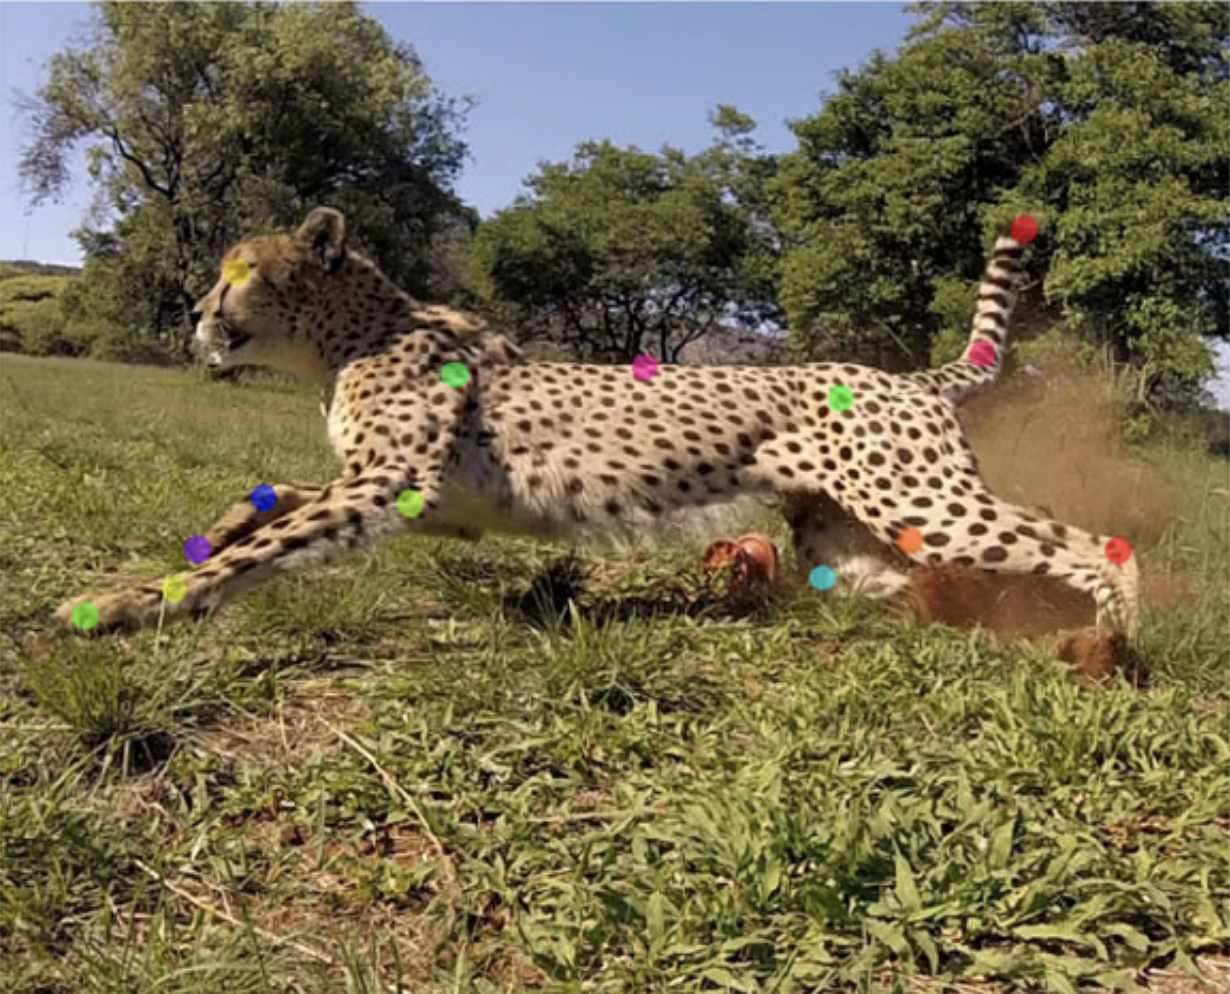
\includegraphics [width=\textwidth/2] {deeplabcut}
  \caption{Предсказанный кадр DeepLabCut} 
  \label{img:deeplabcut}  
\end{figure}
Ограничениями данного метода являются необходимость в разметке этих первых 200 кадров, на это уходит обычно около 20 минут, а также принципиальная возможность работать только с видеопотоком. 
В итоге это достаточно хороший метод для того чтобы разметить большие видеопотоки. Алгоритм обеспечивает достаточную точность и на длинных видеозаписях позволяет сильно сократить время на разметку данных для Pose Tree Estimation. Применение данного способа не ограничивается только на животных: любой видеопоток, на котором можно отслеживать объекты будет работать.

\section{Разметка данных} \label{sect1_4}
Обязательным процессом любой задачи связанной с машинным обучением является получение и разметка данных. Разметкой данных в зависимости от объёма можно заниматься как самостоятельно, так и с помощью наёмного труда. 

\subsection{Самостоятельная разметка данных} \label{subsect1_3_1}
Нет ничего страшного в том чтобы разметить несколько тысяч изображений. Практика показывает, что на самостоятельную разметку тысячи изображений при наличии необходимых инструментов уходит от 20 минут до часа.

К достоинствам самостоятельной разметки можно отнести:
\begin{itemize}
    \item Надёжность - возможность полностью контролировать результат
    \item Независимость - нет нужды полагаться на других людей или сервисы
    \item Дешевизна - не нужно никому платить
    \item Возможность ознакомится с набором данных
\end{itemize}
И действительно, ознакомившись с набором данных, можно увидеть его недостатки, или наоборот, особенности, которые могут помочь решить задачу.

Недостатки:
\begin{itemize}
    \item Разметка больших наборов данных изнуряет
    \item Это самый медленный способ получить данные
    \item Часто приходится создавать инструменты для разметки самостоятельно
\end{itemize}


\subsection{Разметка данных с помощью сторонних сервисов} \label{subsect1_4_2}
Когда самостоятельная разметка невозможна или занимает слишком много времени, можно воспользоваться специальными сервисами для разметки данных. Такими являются Яндекс.Толока и Amazon Mechanical Turk.

Достоинства:
\begin{itemize}
    \item Скорость - из-за большого количества пользователей на разметку даже больших датасетов редко уходит больше часа.
    \item Встроенные в сервисы инструменты для разметки
    \item Относительная дешевизна.
\end{itemize}
Недостатки:
\begin{itemize}
    \item Качество разметки крайне низкое
    \item Для сложных заданий требуется составлять обучение
    \item Требуется опыт в составлении заданий на платформе
    \item Невозможность разметки коммерчески секретных данных
\end{itemize}
Главным недостатком таких сервисов является то, что пользователи не знают ничего о задаче автора. Поэтому задания надо составлять максимально точно, и заставлять пользователей проходить обучение прежде чем решать задачу. Более того, часть пользователей могут вместо правильных ответов давать быстрые, и за этим тоже необходимо следить.

\subsection{Разметка данных с помощью наёмного штата} \label{subsect1_3_3}
Обычно, серьёзные команды на рынке машинного обучения для разметки данных используют собственные наёмные команды.

Достоинства:
\begin{itemize}
    \item Высокое качество разметки
    \item Возможность получать обратную связь
    \item Возможность лично и устно формулировать задания штату
    \item Возможность подписать соглашение о неразглашении
\end{itemize}
Недостатки:
\begin{itemize}
    \item Цена. Это самый дорогой способ
\end{itemize}
Часто такие команды нанимают под однотипные задачи. Например, если есть постоянный поток данных с камер автомобилей, такая команда может размечать данные специально для компании. В таком случае можно обеспечить постоянную нагрузку на штат, а сотрудники будут опытными в решении задачи.